\section{Микрораспределение {\it Macoma balthica}}	
Описание микрораспределения макробентоса проводили при помощи метода пространственных автокорреляций с использованием индекса Морана (\cite{Thrush_et_al_1989}).

\subsection{Восточный Мурман}
На Восточном Мурмане в 2007 году были проведены исследования микрораспределения маком на двух учаcтках --- в куту губы Ярнышная (рис.~\ref{ris:MoranI_Yarnyshnaya}) и на Дальнем пляже губы Дальнезеленецкой (рис.~\ref{ris:MoranI_DZ_2007}). 
На обоих участках не было обнаружено пятен агрегации, связанных с распределением моллюсков по численности или биомассе.
%
	\begin{figure}[h]
	\begin{minipage}[b]{.46\linewidth}
	%Фигурка в первом ряду слева размер отведенный под весь этот объект -- 0.46 от ширины строки
	%Параметр [b] означает, что выравнивание этих министраниц будет по нижнему краю
	\begin{center}
	{\small N}\\
	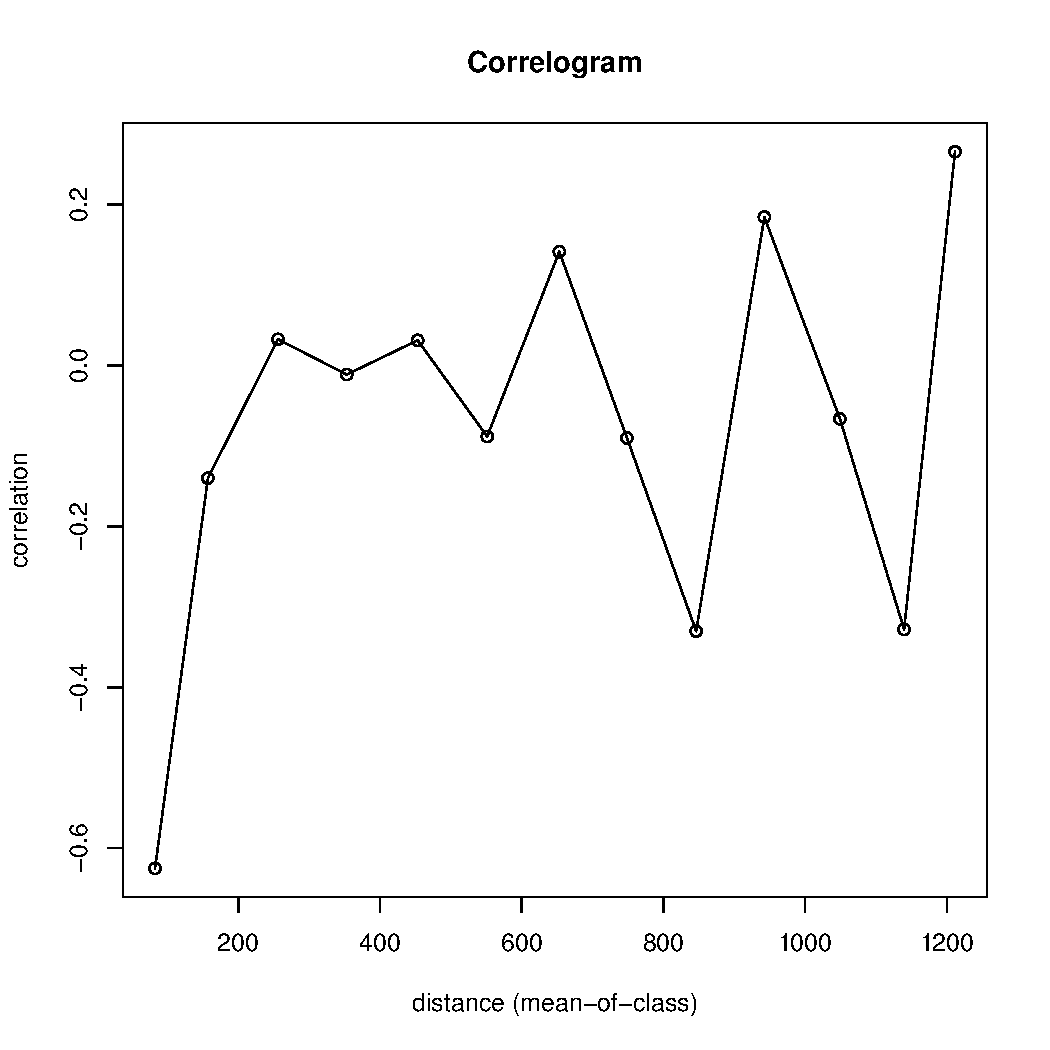
\includegraphics[width=80mm]{../Barenc_Sea/distribution_Moran/Yarnyshnaya07_moran_N_Macoma_balthica_.pdf}
	\end{center}
	\end{minipage}
%
	\hfil %Это пружинка отодвигающая рисунки друг от друга
%
	\begin{minipage}[b]{.46\linewidth}
%Следующий рисунок - первый ряд справа %DUNGEON S_4 \ AB
	\begin{center}
	{\small B}\\
		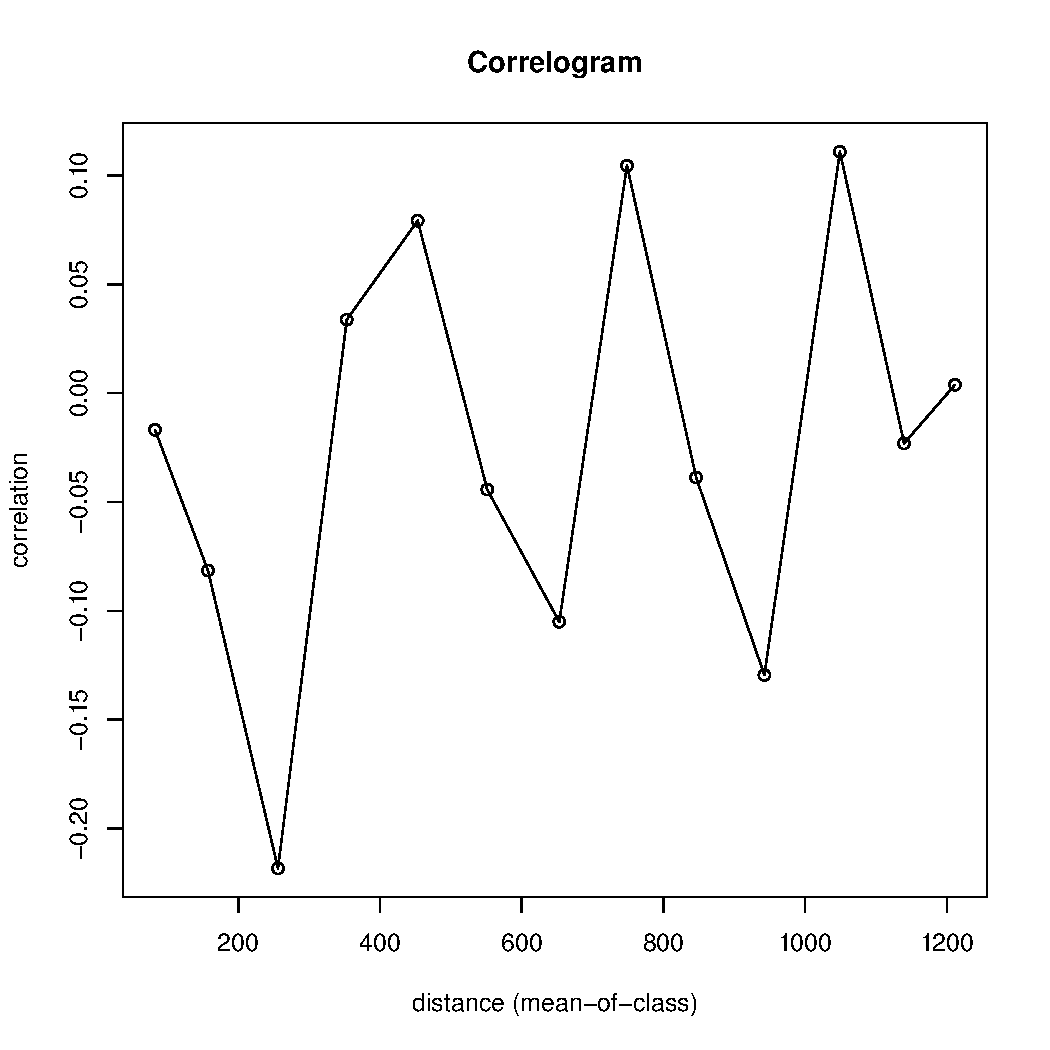
\includegraphics[width=80mm]{../Barenc_Sea/distribution_Moran/Yarnyshnaya07_moran_B_Macoma_balthica_.pdf}
	\end{center}
	\end{minipage}
	
	\begin{minipage}[b]{.46\linewidth}
	%Фигурка в первом ряду слева размер отведенный под весь этот объект -- 0.46 от ширины строки
	%Параметр [b] означает, что выравнивание этих министраниц будет по нижнему краю
	\begin{center}
		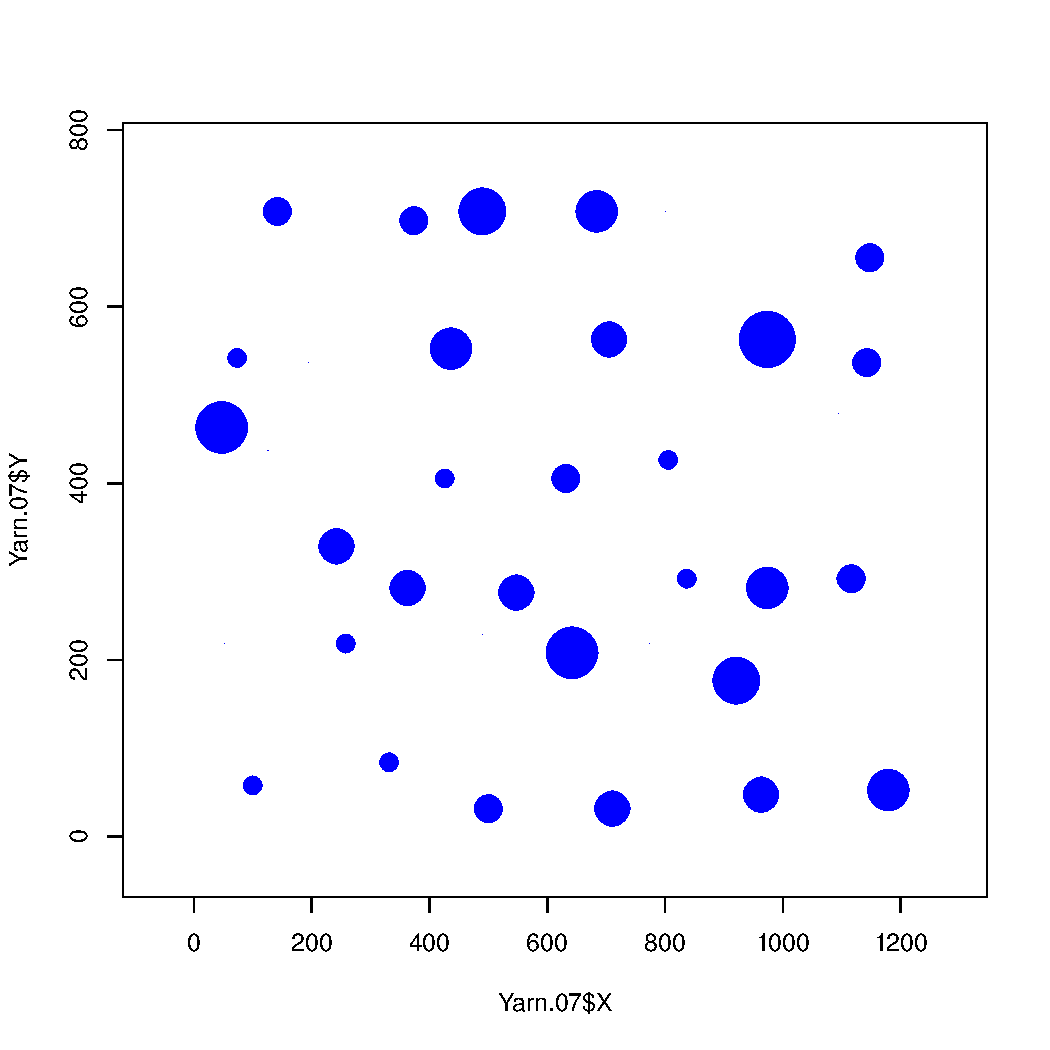
\includegraphics[width=80mm]{../Barenc_Sea/distribution_Moran/Yarnyshnaya_N_Macoma_bubbles.pdf}
	\end{center}
	\end{minipage}
	%
	\hfil %Это пружинка отодвигающая рисунки друг от друга
	%
	\begin{minipage}[b]{.46\linewidth}
%Следующий рисунок - первый ряд справа %DUNGEON S_4 \ AB
	\begin{center}
		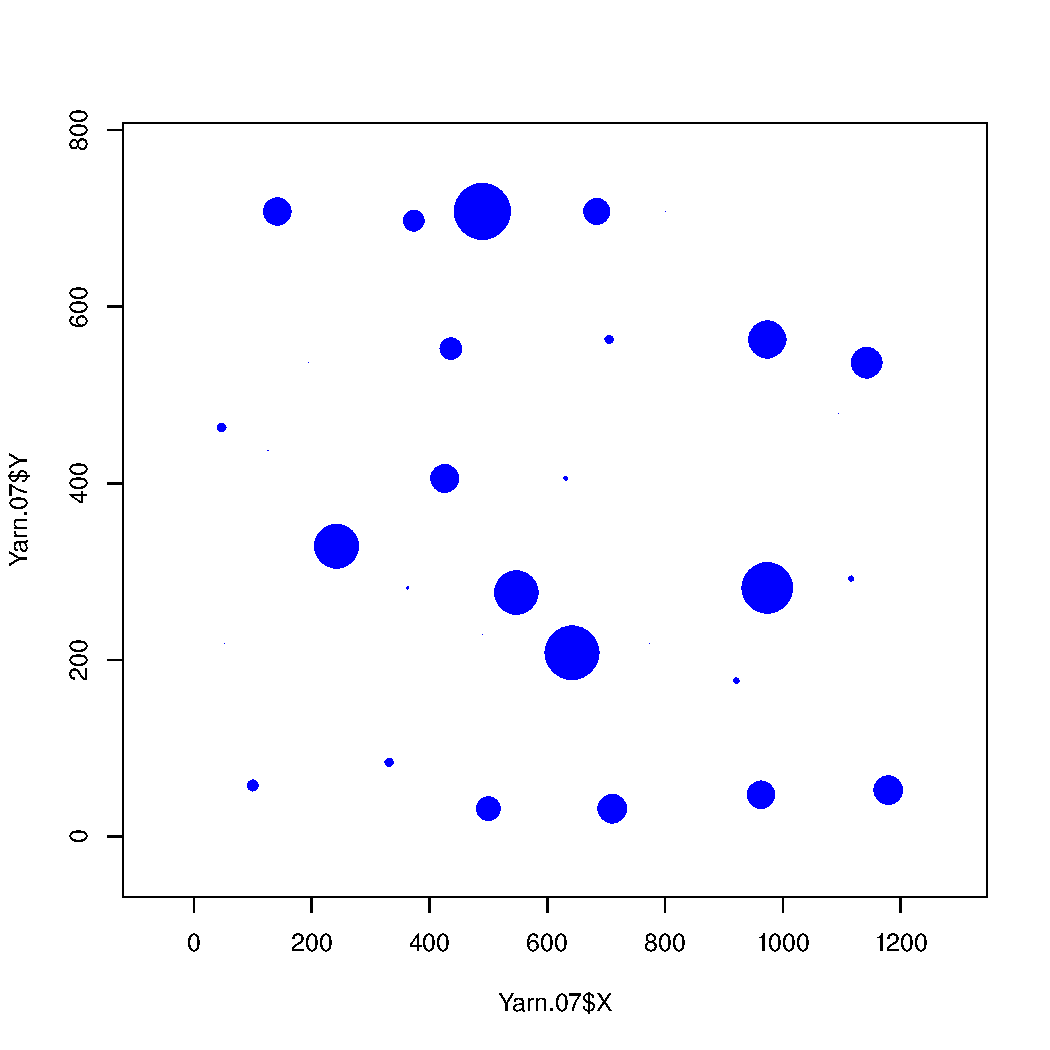
\includegraphics[width=80mm]{../Barenc_Sea/distribution_Moran/Yarnyshnaya_B_Macoma_bubbles.pdf}
	\end{center}
	\end{minipage}
	\caption{Коррелограммы Морана, описывающие микрораспределение, и реальное распределение {\it Macoma balthica} на литорали губы Ярнышная}
	\label{ris:MoranI_Yarnyshnaya}

	\footnotesize{Примечание: N --- распределение особей по численности. B -- распределение особей по биомассе.\\
	Moran's I --- коэффициент пространственной автокорреляции Морана. lag --- расстояние,~см. Закрашенные точки соответстсвуют достоверным значениям коэффициента корреляции ($p \le 0,05$).\\
	На пузырьковых диаграммах площадь кругов пропорциональна обилию маком.}
	\end{figure}



	\begin{figure}[h]

	\begin{minipage}[b]{.46\linewidth}
%Фигурка в первом ряду слева размер отведенный под весь этот объект -- 0.46 от ширины строки
%Параметр [b] означает, что выравнивание этих министраниц будет по нижнему краю
	\begin{center}
	{\small N}\\
		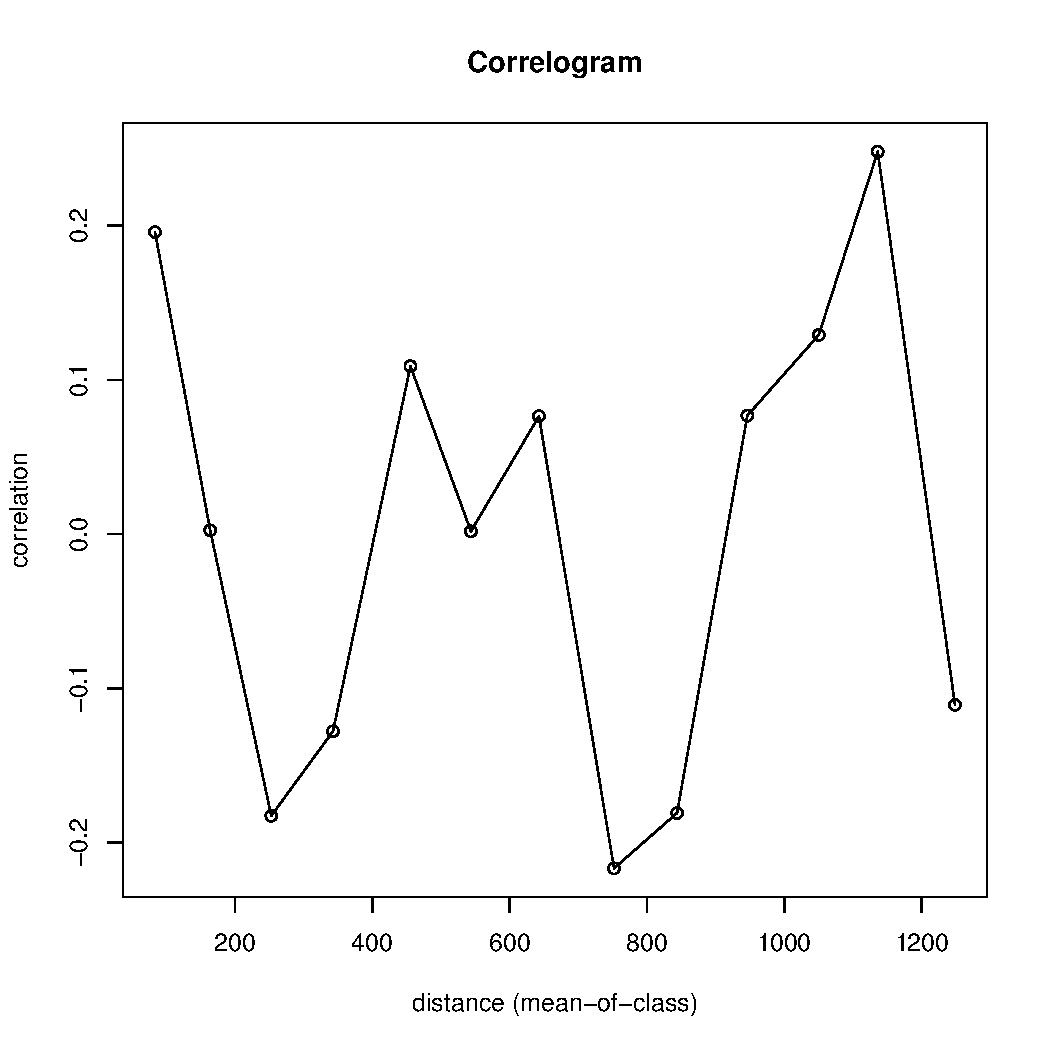
\includegraphics[width=80mm]{../Barenc_Sea/distribution_Moran/Plyazh07_moran_N_Macoma_balthica_.pdf}
	\end{center}
	\end{minipage}
%
	\hfil %Это пружинка отодвигающая рисунки друг от друга
%
	\begin{minipage}[b]{.46\linewidth}
%Следующий рисунок - первый ряд справа %DUNGEON S_4 \ AB
	\begin{center}
	{\small B}\\
		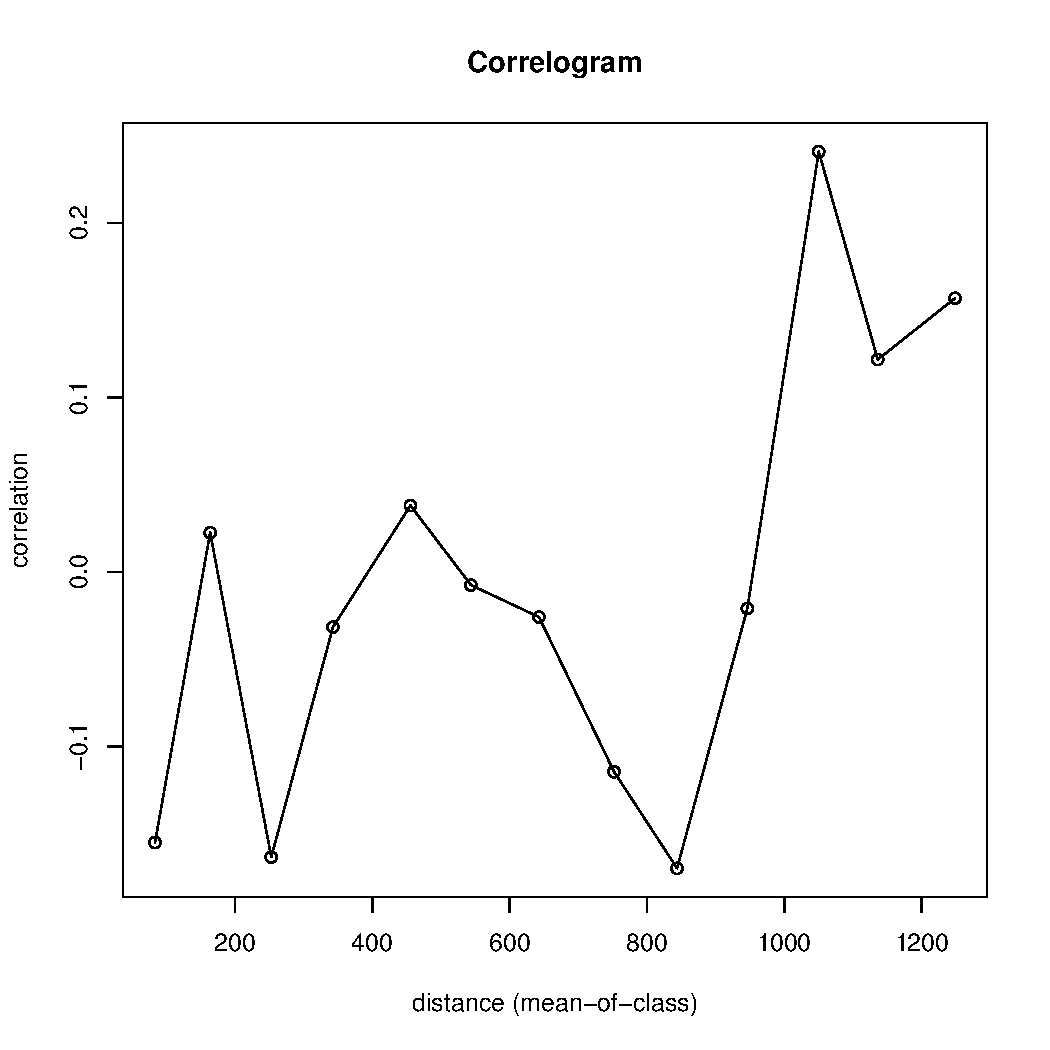
\includegraphics[width=80mm]{../Barenc_Sea/distribution_Moran/Plyazh07_moran_B_Macoma_balthica_.pdf}
	\end{center}
	\end{minipage}
	
	\begin{minipage}[b]{.46\linewidth}
	%Фигурка в первом ряду слева размер отведенный под весь этот объект -- 0.46 от ширины строки
	%Параметр [b] означает, что выравнивание этих министраниц будет по нижнему краю
	\begin{center}
		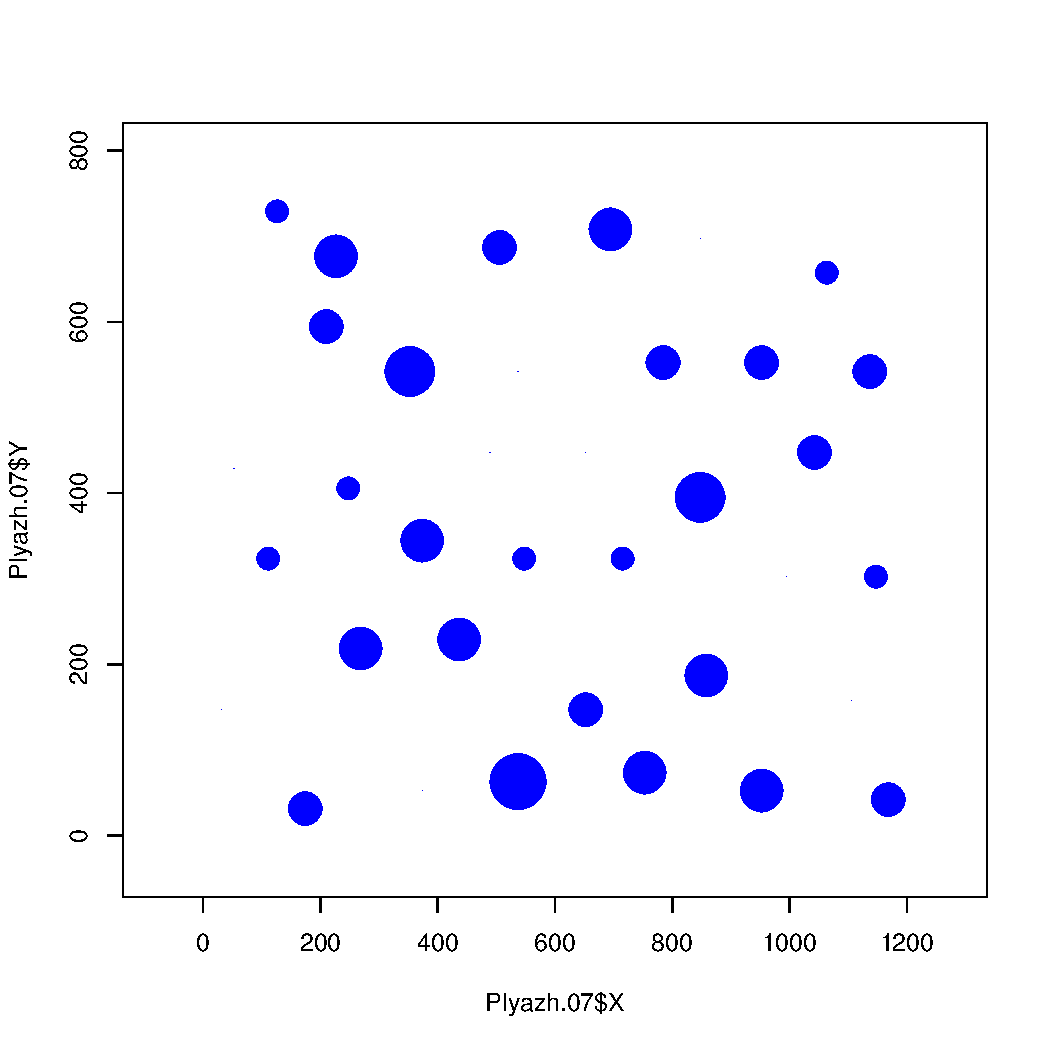
\includegraphics[width=80mm]{../Barenc_Sea/distribution_Moran/Plyazh07_N_Macoma_bubbles.pdf}
	\end{center}
	\end{minipage}
	%
	\hfil %Это пружинка отодвигающая рисунки друг от друга
	%
	\begin{minipage}[b]{.46\linewidth}
%Следующий рисунок - первый ряд справа %DUNGEON S_4 \ AB
	\begin{center}
		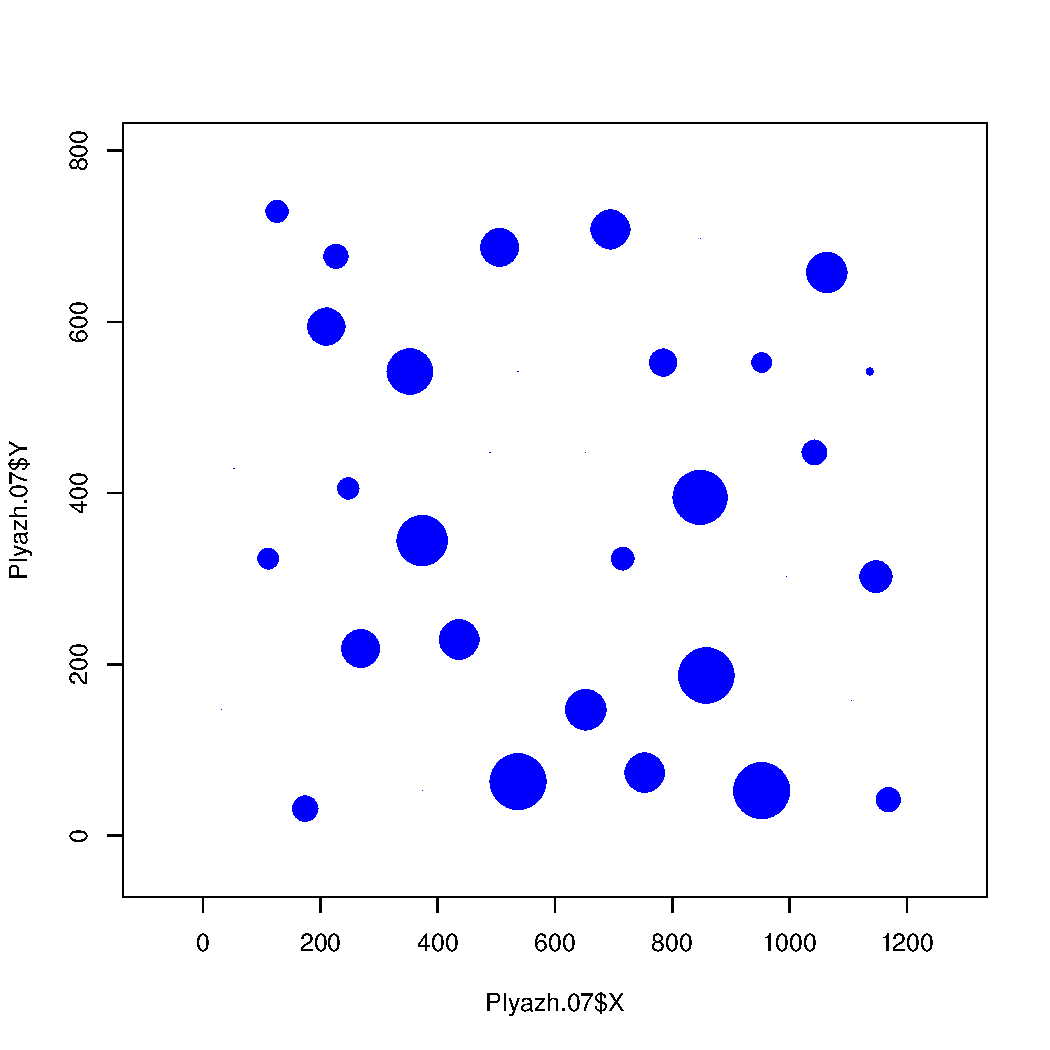
\includegraphics[width=80mm]{../Barenc_Sea/distribution_Moran/Plyazh07_B_Macoma_bubbles.pdf}
	\end{center}
	\end{minipage}
	\caption{Коррелограммы Морана, описывающие микрораспределение, и реальное распределение {\it Macoma balthica} на литорали губы Дальнезеленецкая в 2007 году}
	\label{ris:MoranI_DZ_2007}

	\footnotesize{Примечание: N --- распределение особей по численности. B -- распределение особей по биомассе.\\
	Moran's I --- коэффициент пространственной автокорреляции Морана. lag --- расстояние,~см. Закрашенные точки соответстсвуют достоверным значениям коэффициента корреляции ($p \le 0,05$).\\
	На пузырьковых диаграммах площадь кругов пропорциональна обилию маком.}
	\end{figure}

Мы предположили, что размер учетного полигона слишком маленький для выявления особенностей распределения, и в 2008 году повторили съемку, увеличив размер полигона и количество проб в два раза.
Достоверные значения коэффициента простарнственной корреляции Морана были показаны для расстояний около $1,5-2$~м (отрицательный) и на расстоянии около $4$~м (положительный) (рис.~\ref{ris:MoranI_DZ_2008}).
%
	\begin{figure}[h]

	\begin{minipage}[b]{.46\linewidth}
%Фигурка в первом ряду слева размер отведенный под весь этот объект -- 0.46 от ширины строки
%Параметр [b] означает, что выравнивание этих министраниц будет по нижнему краю
	\begin{center}
	{\small N}\\
		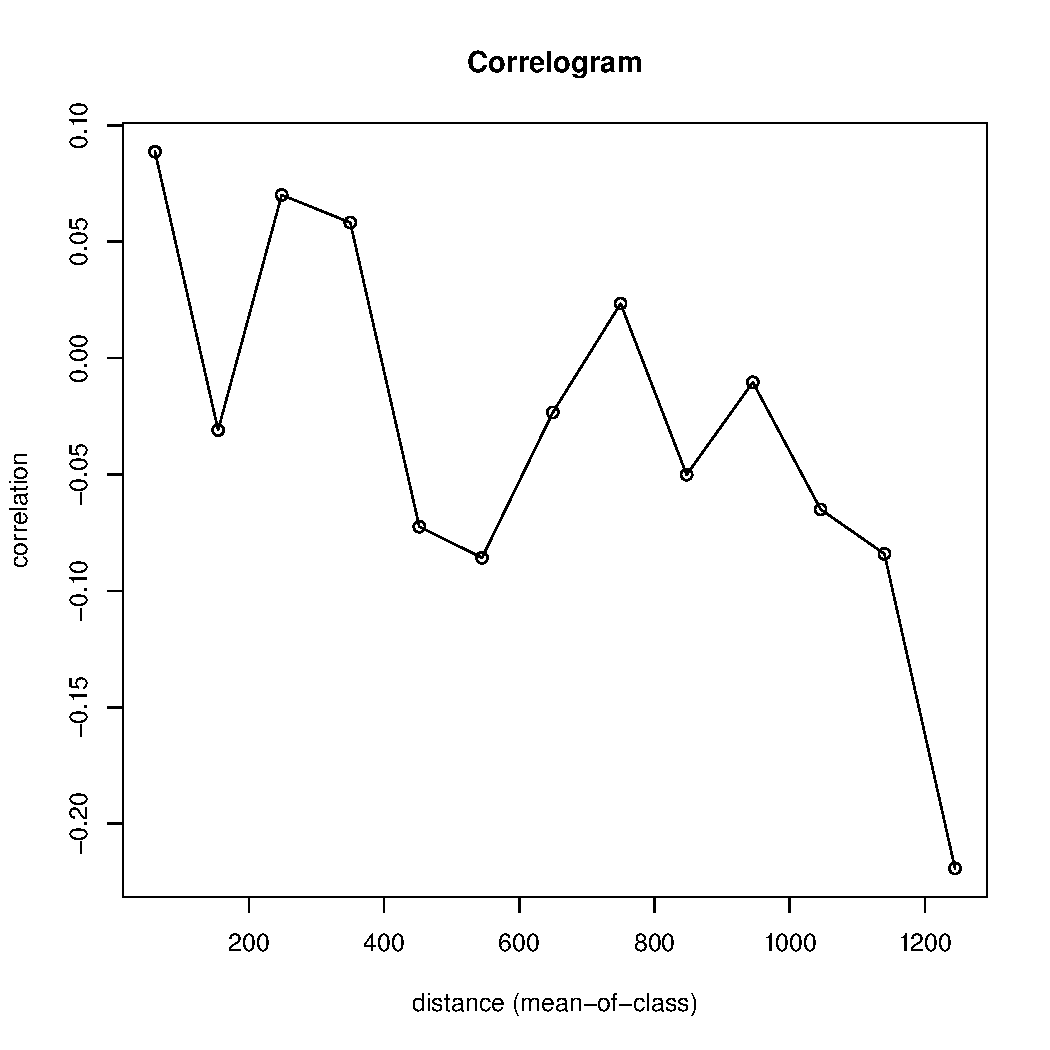
\includegraphics[width=80mm]{../Barenc_Sea/distribution_Moran/Plyazh0812_moran_N_Macoma_balthica_.pdf}
	\end{center}
	\end{minipage}
%
	\hfil %Это пружинка отодвигающая рисунки друг от друга
%
	\begin{minipage}[b]{.46\linewidth}
%Следующий рисунок - первый ряд справа %DUNGEON S_4 \ AB
	\begin{center}
	{\small B}\\
		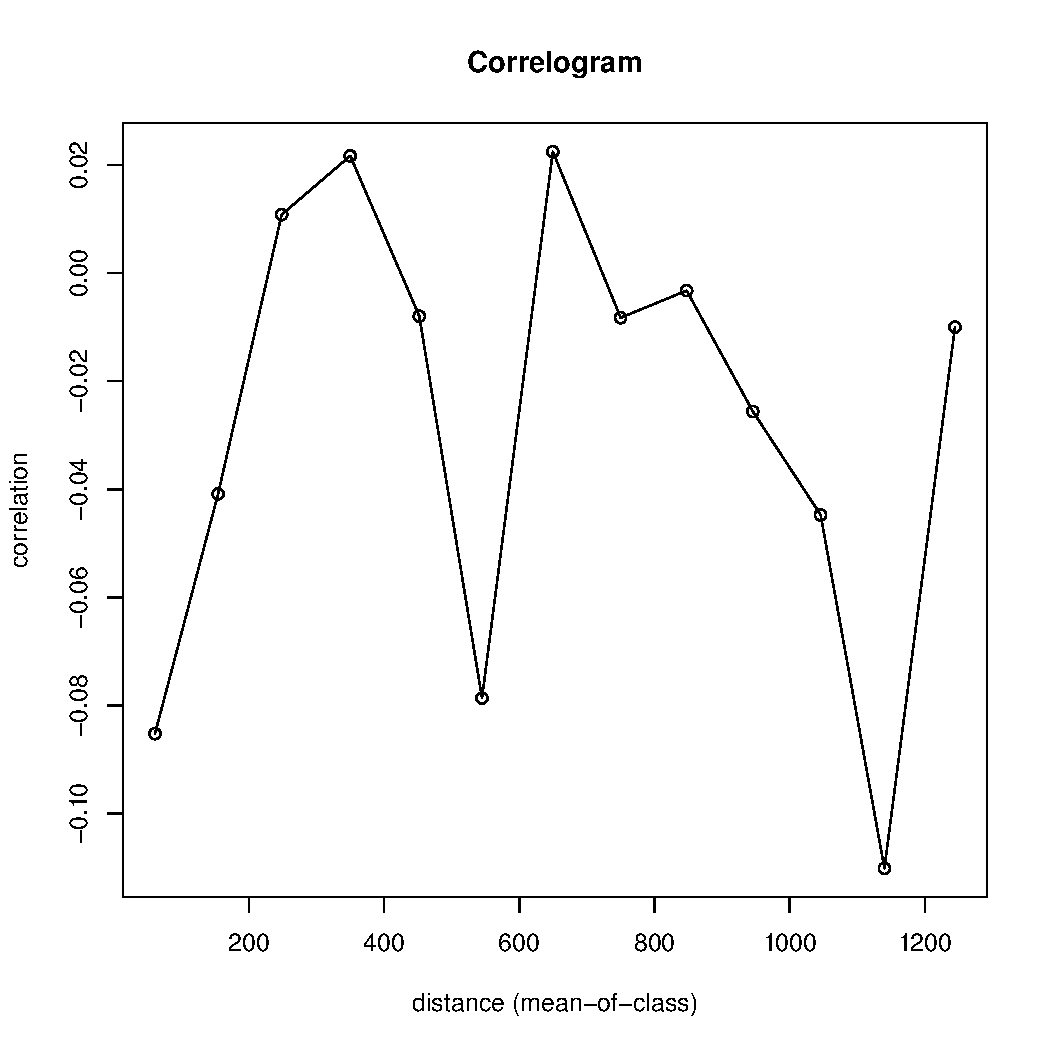
\includegraphics[width=80mm]{../Barenc_Sea/distribution_Moran/Plyazh0812_moran_B_Macoma_balthica_.pdf}
	\end{center}
	\end{minipage}
	
	\begin{minipage}[b]{.46\linewidth}
	%Фигурка в первом ряду слева размер отведенный под весь этот объект -- 0.46 от ширины строки
	%Параметр [b] означает, что выравнивание этих министраниц будет по нижнему краю
	\begin{center}
		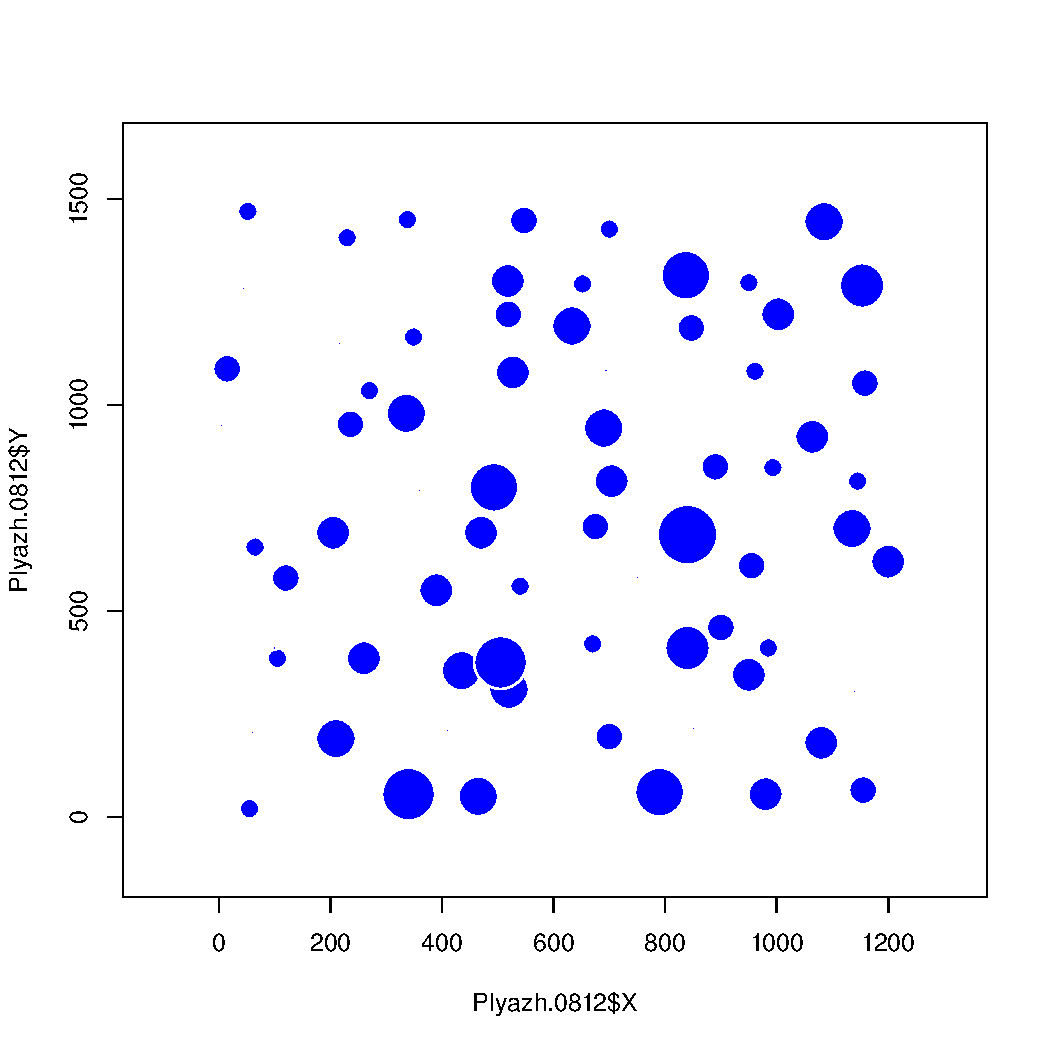
\includegraphics[width=80mm]{../Barenc_Sea/distribution_Moran/Plyazh0812_N_Macoma_bubbles.pdf}
	\end{center}
	\end{minipage}
	%
	\hfil %Это пружинка отодвигающая рисунки друг от друга
	%
	\begin{minipage}[b]{.46\linewidth}
%Следующий рисунок - первый ряд справа %DUNGEON S_4 \ AB
	\begin{center}
		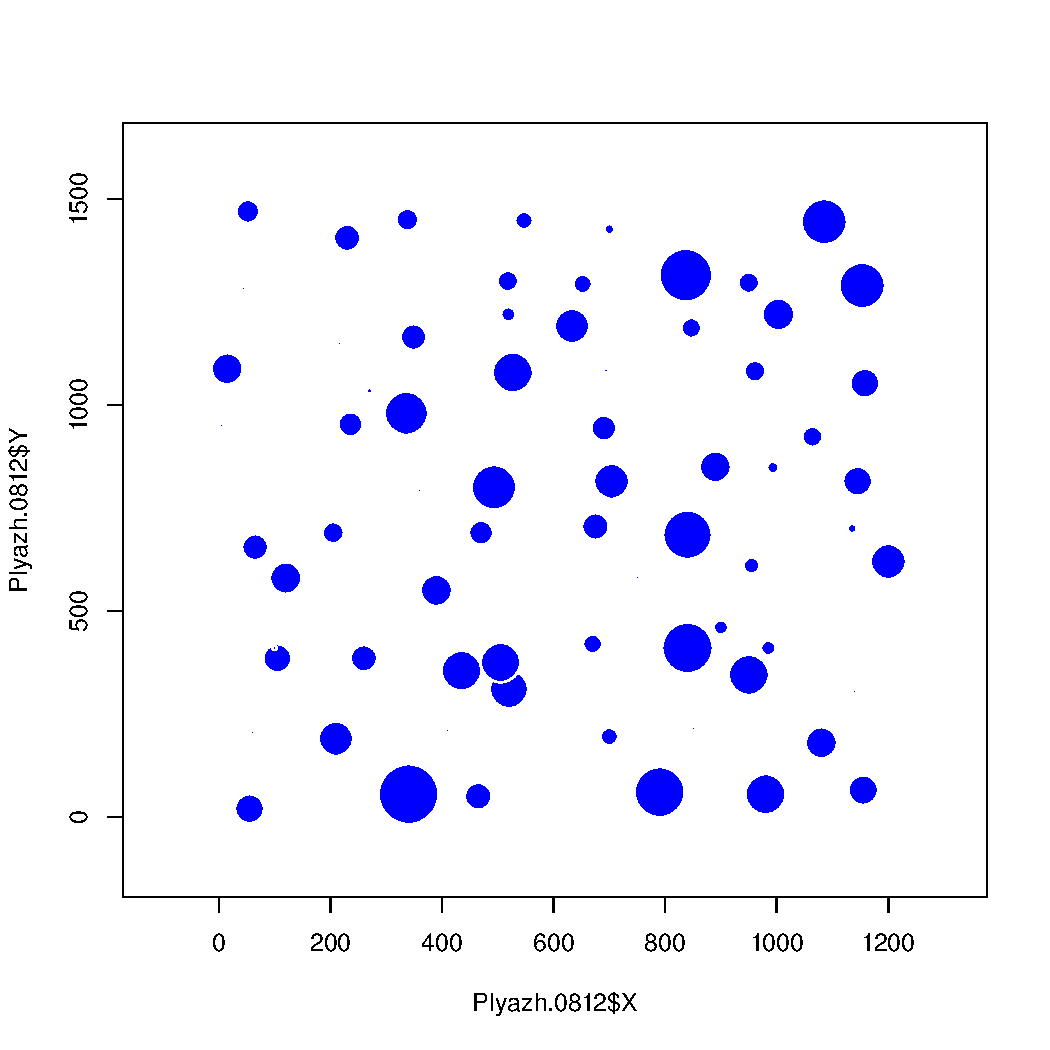
\includegraphics[width=80mm]{../Barenc_Sea/distribution_Moran/Plyazh0812_B_Macoma_bubbles.pdf}
	\end{center}
	\end{minipage}
	\caption{Коррелограммы Морана, описывающие микрораспределение, и реальное распределение {\it Macoma balthica} на литорали губы Дальнезеленецкая в 2008 году}
	\label{ris:MoranI_DZ_2008}

	\footnotesize{Примечание: N --- распределение особей по численности. B -- распределение особей по биомассе.\\
	Moran's I --- коэффициент пространственной автокорреляции Морана. lag --- расстояние,~см. Закрашенные точки соответстсвуют достоверным значениям коэффициента корреляции ($p \le 0,05$).\\
	На пузырьковых диаграммах площадь кругов пропорциональна обилию маком.}
	\end{figure}
%
Это позволяет предположить сложную структуру пространственного распределения особей: локальные агрегации, сравнимые по размеру с размером учетной рамки (1/30 м$^2$), организованные в более крупные скопления. 


	\subsection{Кольский залив}
На литорали Пала-губы особи {\it M.~balthica} формируют скопления размером около $2-4$~м (рис.~\ref{ris:moransI_Pala_Macoma}). 
Наличие серии достоверно отрицательных значений индекса автокорреляции Морана для больших расстояний свидетельствует о наличии либо градиентого изменения численности, либо крупной агрегации с нечеткими краями.
Наличие градиентного изменения обилия в направлении к руслу ручья было показано с использованием коэффициента корреляции Кендалла ($\tau = 0,55; p = 3,48 \times 10^{-6}$).
Распределение маком по биомассе соответствует распределению по численности (рис.~\ref{ris:moransI_Pala_Macoma}). Также корреляционный анализ Кендалла показал градиентное уменьшение биомассы в направлении от моря ($\tau = -0,4; p = 0,0005$).
	\begin{figure}[h]

	\begin{minipage}[b]{.5\linewidth}
	%Фигурка в первом ряду слева размер отведенный под весь этот объект -- 0.46 от ширины строки
	%Параметр [b] означает, что выравнивание этих министраниц будет по нижнему краю
	\begin{center}
	{\small N}\\
		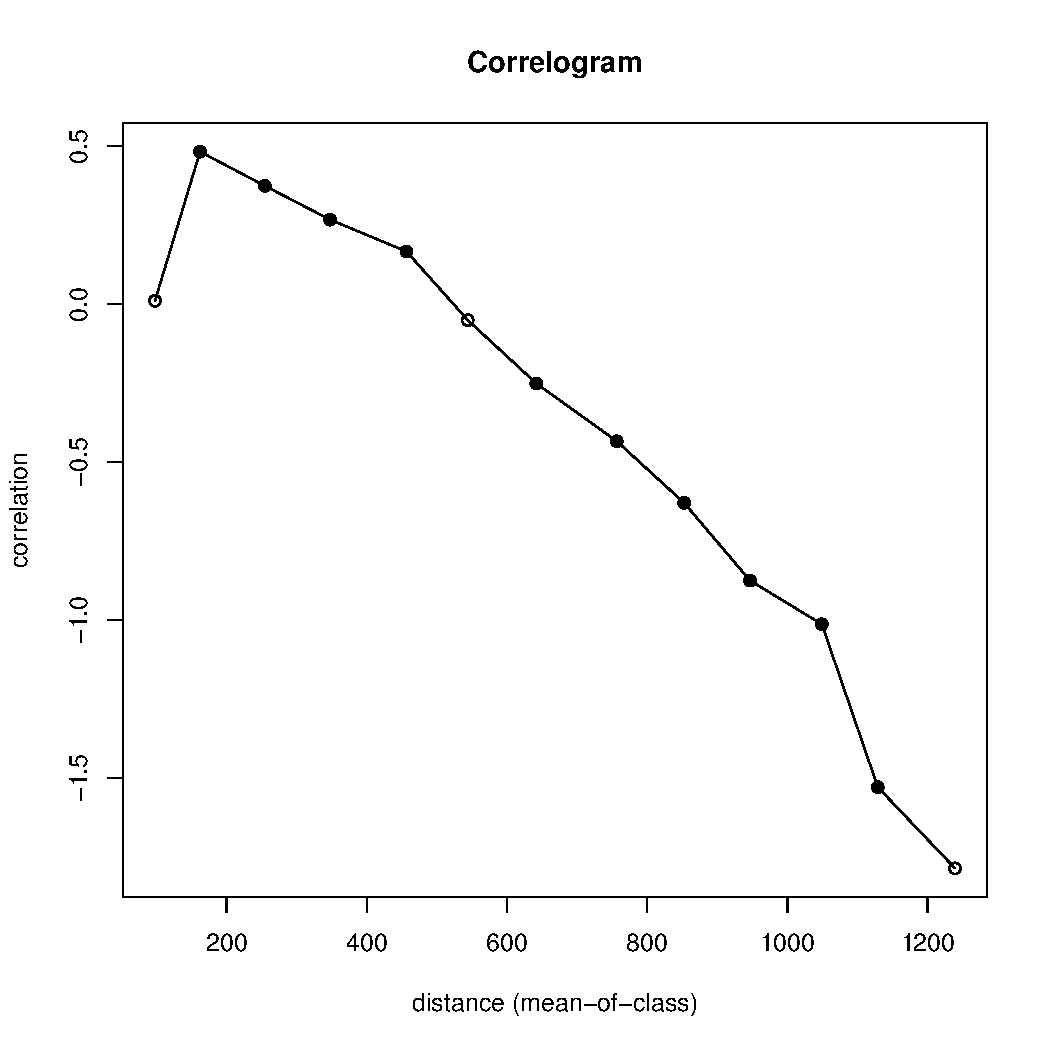
\includegraphics[width=80mm]{../Barenc_Sea/distribution_Moran/Pala_moran_N_Macoma_balthica_.pdf}
	\end{center}
	\end{minipage}
	%
	\hfil %Это пружинка отодвигающая рисунки друг от друга
	%
	\begin{minipage}[b]{.5\linewidth}
	%Следующий рисунок - первый ряд справа %DUNGEON S_4 \ AB
	\begin{center}
	{\small B}\\
		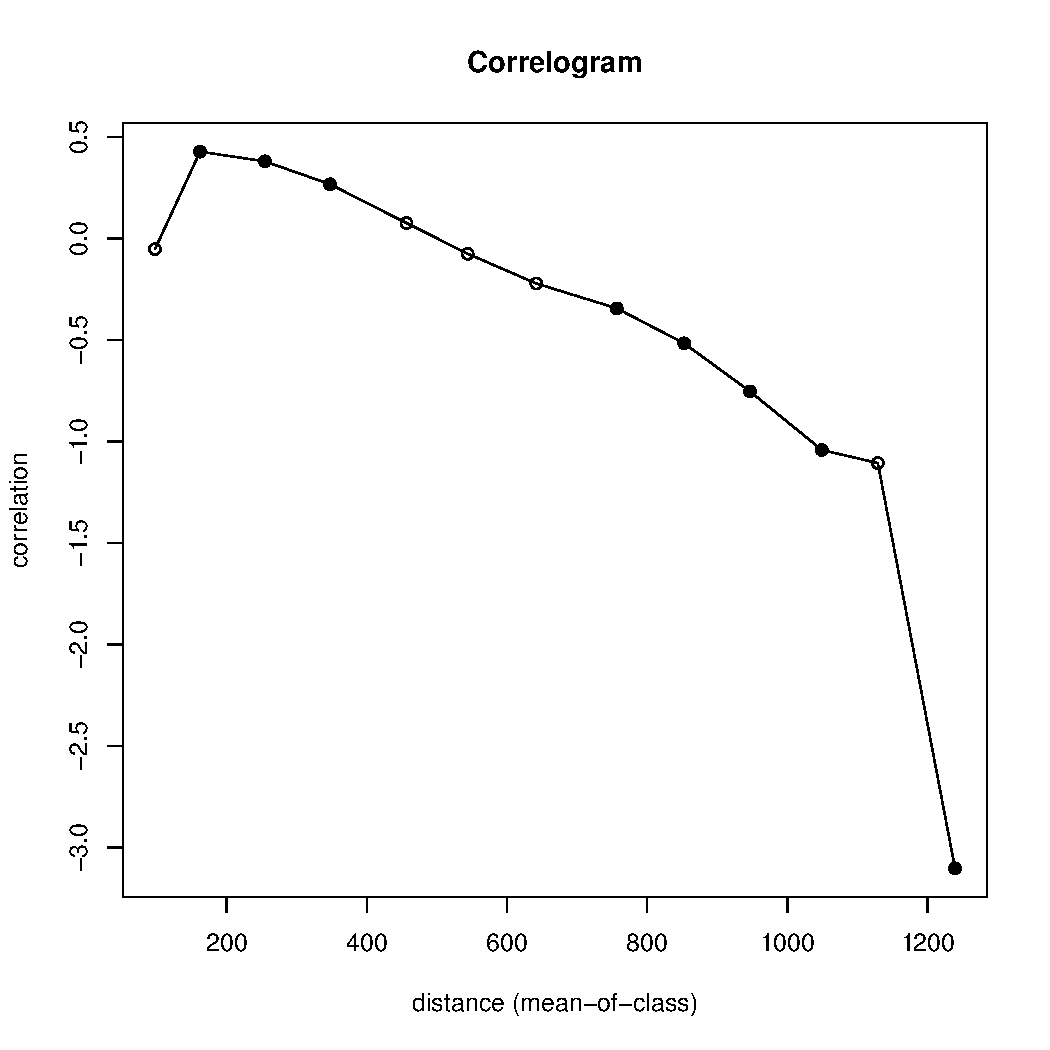
\includegraphics[width=80mm]{../Barenc_Sea/distribution_Moran/Pala_moran_B_Macoma_balthica_.pdf}
	\end{center}
	\end{minipage}

	\begin{minipage}[b]{.5\linewidth}
	\begin{center}
		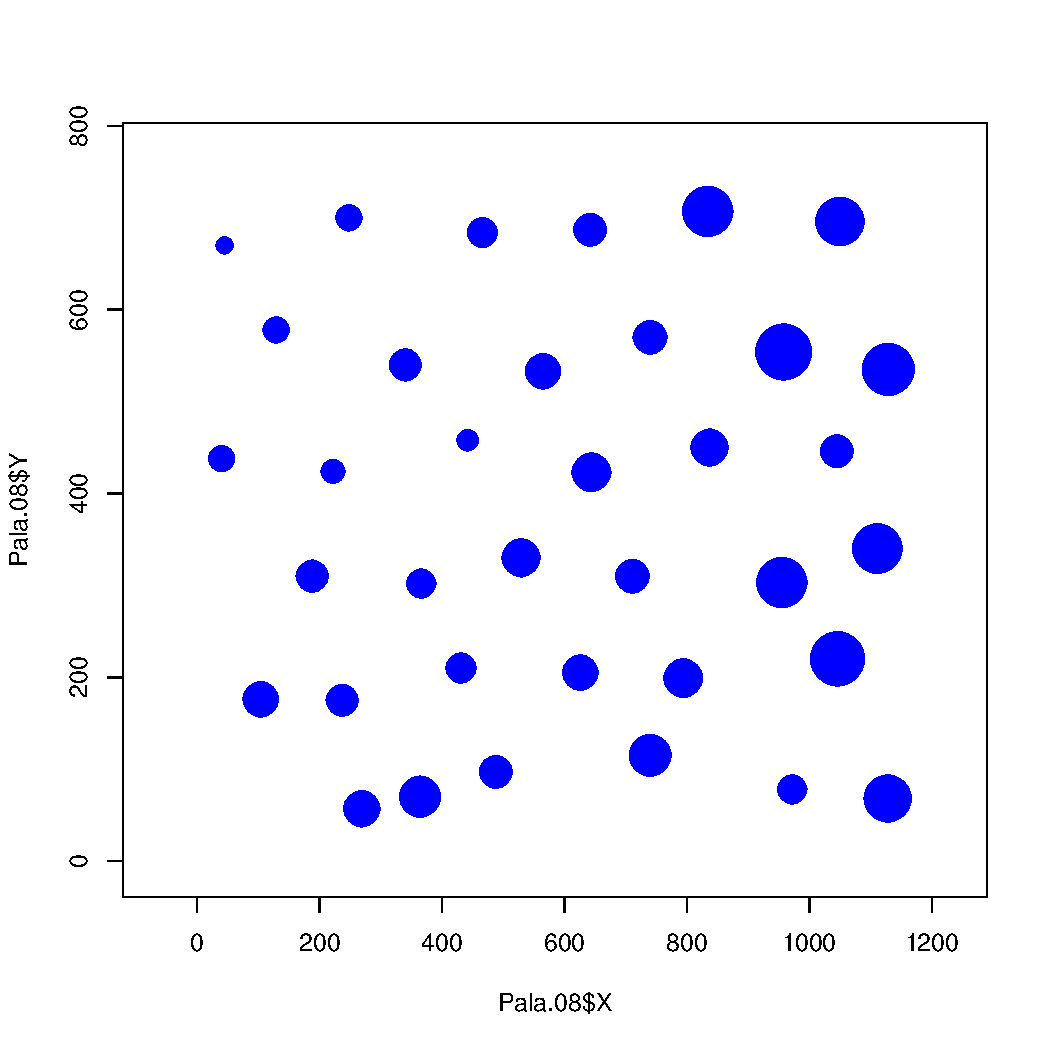
\includegraphics[width=80mm]{../Barenc_Sea/distribution_Moran/Pala_N_Macoma_bubbles.pdf}
	\end{center}
	\end{minipage}
	%
	\hfil %Это пружинка отодвигающая рисунки друг от друга
	%
	\begin{minipage}[b]{.5\linewidth}
	%Следующий рисунок - первый ряд справа %DUNGEON S_4 \ AB
	\begin{center}
		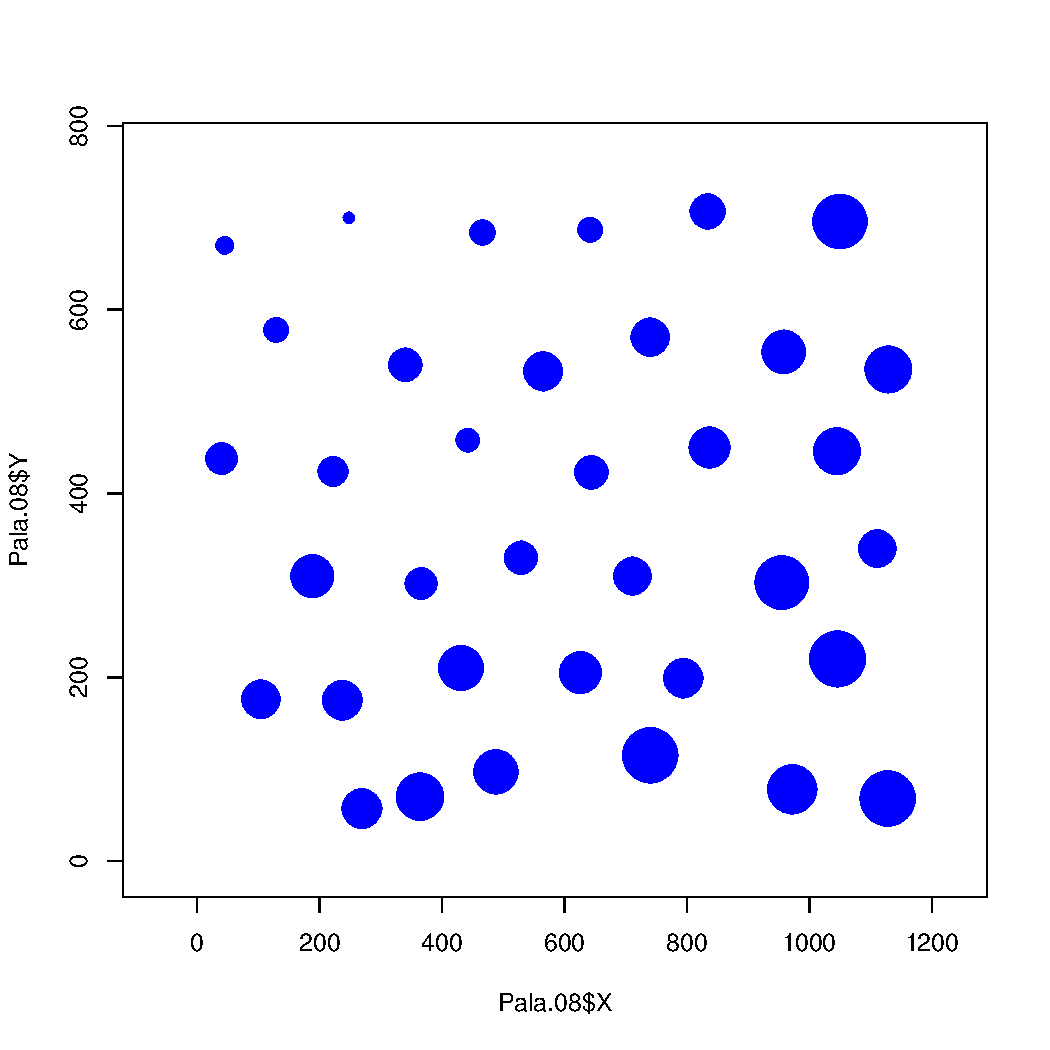
\includegraphics[width=80mm]{../Barenc_Sea/distribution_Moran/Pala_B_Macoma_bubbles.pdf}
	\end{center}
	\end{minipage}
	\caption{Коррелограммы Морана, описывающие микрораспределение, и реальное распределение {\it Macoma balthica} на литорали Пала-губы}
	\label{ris:moransI_Pala_Macoma}

	\footnotesize{Примечание: N --- распределение особей по численности. B -- распределение особей по биомассе.\\
	Moran's I --- коэффициент пространственной автокорреляции Морана. lag --- расстояние,~см. Закрашенные точки соответстсвуют достоверным значениям коэффициента корреляции ($p \le 0,05$).\\
	На пузырьковых диаграммах площадь кругов пропорциональна обилию маком.}
	\end{figure}

Поскольку на данном участке обилие маком было достаточно высокое (рис.~\ref{ris:age_Pala_2007_low}), мы отдельно рассмотрели распределение особей разных возрастов.
%
	\begin{figure}[h]
		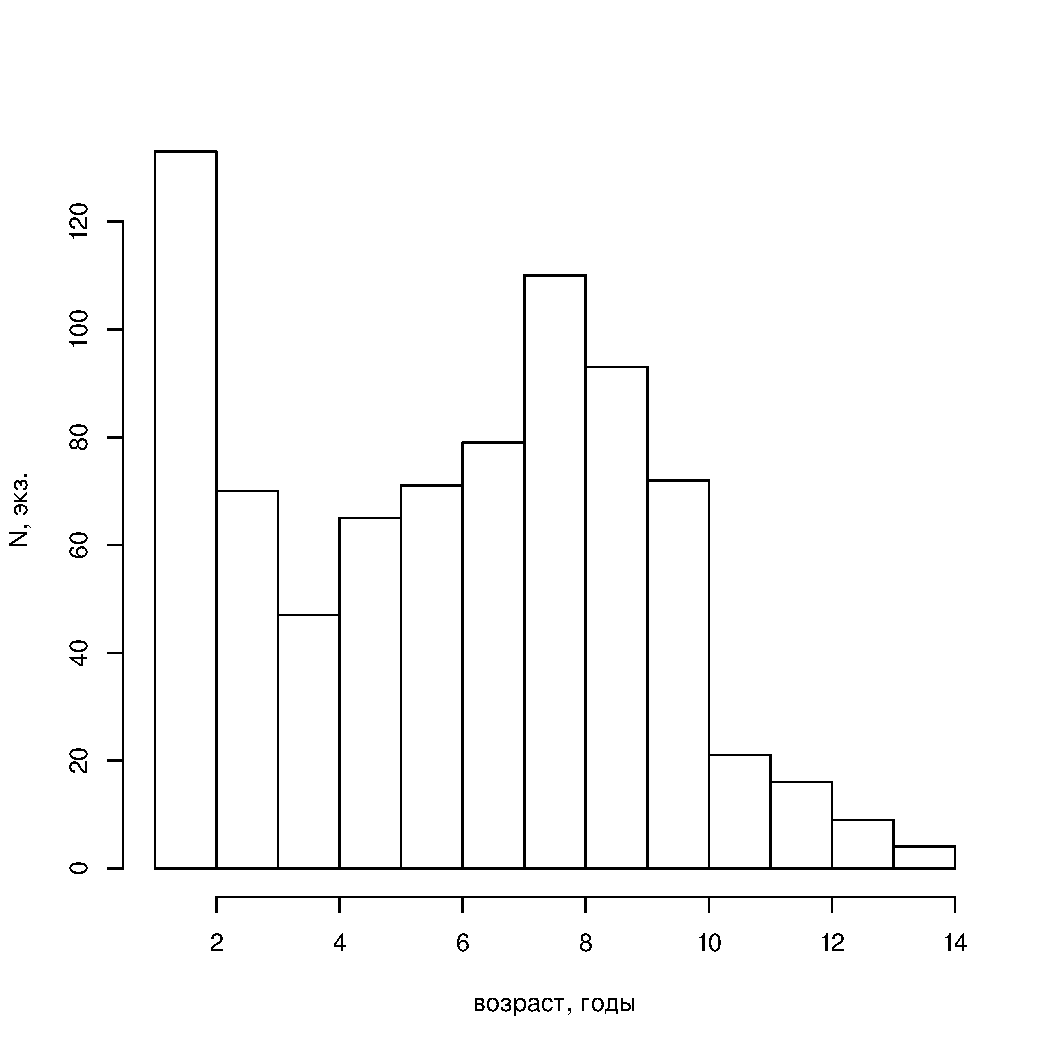
\includegraphics{../Barenc_Sea/Pala/Pala_2007_low_age_hist.pdf}
		\caption{Распределение по возрастам особей {\it Macoma balthica} в пробах на литорали Пала-губы}
		\label{ris:age_Pala_2007_low}
	\end{figure}
%
Коррелограммы Морана и пузырьковые диаграммы, описывающие реальное распределение особей, представлены в приложении \ref{app:Pala_MoranI_ages}.
Было показано, что горизонтальный градиент общего обилия связан в первую очередь с таким распределением особей возрастом 2, 3 и 5 лет (табл.~\ref{tab:Pala_ages_distribution}). 
%
\begin{table}[h]
		\caption{Пространственное распределение особей {\it Macoma balthica} разного возраста}
		\label{tab:Pala_ages_distribution}
\begin{tabularx}{\linewidth}{|c|X|rr|rr|}
\hline
	& распределение		& \multicolumn{2}{c|}{градиент горизонтальный} & \multicolumn{2}{c|}{градиент вертикальный}   \\ \cline{3-6}
возраст  &  по результатам пространственной автокорреляции  & $Kendall\ \tau$ & $p-value$ & $Kendall\ \tau$ & $p-value$				\\ \hline

1+       & случайное                      & $0,2$	&	$0,17$	&	$0,02$	&	$0,9$                            \\
2+       & градиент                       & $0,45$	&	$0,0003$ ***	&	$0,2$	&	$0,07$ **                   \\
3+       & градиент                       & $0,5$	&	$2,4 \times 10^{-5}$ ***	&	$0,3$	&	$0,002$ ***		 \\
4+       & случайное                      & $0,2$	&	$0,07$ **	&	$0,06$	&	$0,6$                            \\
5+       & градиент                       & $0,43$	&	$0,0005$ ***	&	$-0,02$	&	$0,9$                    \\
6+       & случайное                      & $0,2$	&	$0,03$ ***	&	$-0,03$	&	$0,8$                            \\
7+       & одно большое пятно             & $0,02$	&	$0,9$	&	$-0,02$	&	$0,9$                             \\
8+       & одно большое пятно             & $0,3$	&	$0,01$ ***	&	$-0,2$	&	$0,04$ ***                            \\
9+       & одно большое пятно             & $0,3$	&	$0,01$ ***	&	$-0,2$	&	$0,1$                             \\
10+      & агрегации размером 1 и 3 метра & $0,2$	&	$0,1$	&	$-0,2$	&	$0,08$ **                            \\
11+      & одно большое пятно             & $0,26$	&	$0,053$ **	&	$-0,1$	&	$0,3$                             \\
12+      & агрегации размером 6 метров    & $0,1$	&	$0,3$	&	$-0,2$	&	$0,2$                             \\
13+      & случайное                      & $0,1$	&	$0,4$	&	$0,04$	&	$0,7$                              \\
14+      & случайное                      &  $0,09$	&	$0,5$	&	$-0,15$	&	$0,3$                             \\ \hline
	\end{tabularx}
\end{table}
%
Предположения о градиентном распределении особей данных возрастов, полученных в ходе анализа пространственных автокорреляций Морана подтвердились при корреляционном анализе Кендалла (табл.~\ref{tab:Pala_ages_distribution}).
Однако в нескольких случаях, где коррелограммы Морана не показывают градиентного распределения, анализ Кендалла показывает достоверную корреляцию обилия с координатами. 
Однако во всех случаях речь идет о слабой связи (коэффициент корреляции $0,2$).

Резюмируя полученные данные, можно говорить о большем влиянии ручья на более молодых моллюсков.
Особи старших возрастов формируют агрегации размером в несколько метров.
Наиболее старые моллюски остаются в количестве единичных особей и распределены случайно.

